\documentclass{tufte-handout}
\ifxetex
  \usepackage{fontspec}
\else
  \usepackage[utf8]{inputenc}
  \usepackage[T1]{fontenc}
\fi

\usepackage[french]{babel}
\usepackage{fontspec}
\usepackage{amsmath, amsthm, amsfonts}
\usepackage[separate-uncertainty]{siunitx}
\usepackage{xcolor}
\usepackage{tikz}
\usepackage{tikz-cd}
\usepackage[object=vectorian]{pgfornament}
\usepackage{circuitikz}
\usepackage{hyperref}
\usepackage{caption}
\usepackage{booktabs}
\usepackage{mathtools}
\usepackage{longtable}
\usepackage[version=3]{mhchem}
\usepackage{marginnote}
\usepackage[framemethod=tikz]{mdframed}


% Paul Tol's qualitative palette
% ``bright''.https://personal.sron.nl/~pault/#sec:qualitative
\definecolor{tblue}{HTML}{4477AA}
\definecolor{tcyan}{HTML}{66CCEE}
\definecolor{tgreen}{HTML}{228833}
\definecolor{tyellow}{HTML}{CCBB44}
\definecolor{tred}{HTML}{EE6677}
\definecolor{tpurple}{HTML}{AA3377}
\definecolor{tgrey}{HTML}{BBBBBB}


% Justification for marginnotes.
\renewcommand*{\raggedleftmarginnote}{}
\renewcommand*{\raggedrightmarginnote}{}


% Styles for mdframed environments.
\newmdenv[backgroundcolor=tgreen!10,linecolor=tgreen!30]{reponsebox}
\newmdenv[backgroundcolor=tyellow!10,linecolor=tyellow!30]{diapobox}
\newmdenv[backgroundcolor=tred!10,linecolor=tred!30]{fondamentalbox}

% Default arrow for tikz and style for positive and negative objects.
\tikzset{>=latex,
    negative/.style={draw=teal!70!black, fill=teal!10, thick},
    positive/.style={draw=red, fill=red!10, thick}}
\usetikzlibrary{matrix,calc,decorations.pathreplacing,decorations.pathmorphing,decorations.markings}

% French locale for numbers and negative exponent for units.
\sisetup{locale=FR, per-mode=symbol}

\newcommand{\abs}[1]{\left| #1 \right|}
\newcommand{\rhat}{\vec{\hat{r}}}
\newcommand{\xhat}{\vec{\imath}}
\newcommand{\yhat}{\vec{\jmath}}
\newcommand{\zhat}{\vec{k}}
\newcommand{\real}{\mathbb{R}}
\newcommand{\der}[2]{\frac{\mathrm{d}#1}{\mathrm{d}#2}}
\newcommand{\pder}[2]{\frac{\partial\ #1}{\partial\ #2}}
\newcommand{\dif}{\mathrm{d}}
\newcommand{\ddif}{\,\mathrm{d}}
\newcommand{\grad}{\vec{\nabla}}
\newcommand{\exemple}[1]{\begin{fullwidth}#1\end{fullwidth}}
\newcommand{\norm}[1]{\lVert\ #1\ \rVert}
\newcommand{\vu}{\vec{u}}
\newcommand{\vv}{\vec{v}}
\newcommand{\vr}{\vec{r}}
\newcommand{\va}{\vec{a}}
\newcommand{\vF}{\vec{F}}
\newcommand{\vE}{\vec{E}}
\newcommand{\vB}{\vec{B}}
\newcommand{\vecxyz}[3]{#1 \xhat\ + #2 \yhat\ + #3 \zhat}
\newcommand{\vecxy}[2]{#1 \xhat\ + #2 \yhat}
\newcommand{\coulombcst}{k}
\newcommand{\emf}{\ensuremath{\mathcal{E}}}
\newcommand{\eval}{\SI{1.602e-19}{C}}
\newcommand{\kval}{\SI{8.99e9}{Nm^2 \per C^2}}

% Nice separator line
\newcommand{\sectionline}{
    \noindent
    \begin{center}
        \resizebox{0.5\linewidth}{1ex}
    {{%
    {\begin{tikzpicture}
    \node  (C) at (0,0) {};
    \node (D) at (9,0) {};
    \path (C) to [ornament=85] (D);
    \end{tikzpicture}}}}
    \end{center}
}

\theoremstyle{definition}
\newtheorem*{defn}{Definition}


\usepackage{textpos}

\sisetup{locale=FR, per-mode=symbol}

% This is necessary to fix tufte-handout when compiling with XeLaTeX.
\ifxetex
  \newcommand{\textls}[2][5]{%
    \begingroup\addfontfeatures{LetterSpace=#1}#2\endgroup
  }
  \renewcommand{\allcapsspacing}[1]{\textls[15]{#1}}
  \renewcommand{\smallcapsspacing}[1]{\textls[10]{#1}}
  \renewcommand{\allcaps}[1]{\textls[15]{\MakeTextUppercase{#1}}}
  \renewcommand{\smallcaps}[1]{\smallcapsspacing{\scshape\MakeTextLowercase{#1}}}
  \renewcommand{\textsc}[1]{\smallcapsspacing{\textsmallcaps{#1}}}
\fi


\title{Exercices sur le travail et l'énergie potentielle}
\date{}
%\author{203-NYB-05 Électricité et magnétisme}


\begin{document}

\maketitle

On déplace un électron du point $A$ au point $B$ tel qu'illustré ci-contre.
L'électron se trouve dans un champ électrique uniforme de \SI{20000}{N/C}.

\begin{marginfigure}
  \begin{tikzpicture}
    \node (A) at (1, 0) {$A$};
    \node (B) at (1, 2) {$B$};
    \node (C) at (0, 1) {$C$};
    \draw[dotted] (A) -- node[right] {$1$} (B);
    \draw[densely dashed] (A) -- (C) -- node[anchor=south east] {$2$} (B);
    \draw[thick, ->] (2, 0.5) -- (2, 1.5) node[right] {$\vec{E}$};
    \draw[|<->|] (-1, 0) -- node[fill=white] {\SI{2}{cm}} (-1, 2);
    \draw[|<->|] (0, -0.5) -- node[fill=white] {\SI{1}{cm}} (1, -0.5);
  \end{tikzpicture}
\end{marginfigure}

\begin{enumerate}
  \item On déplace l'électron en ligne droite de $A$ à $B$ (trajectoire 1),
    déterminez le travail fait par la force électrique sur l'électron.

    \marginnote{Rappel: le travail est définit comme le produit scalaire du
      déplacement et de la force
      \[W = \vec{F} \cdot \Delta\vec{r}\]
    }

  \item On déplace l'électron en ligne droite de $A$ à $C$, puis de $C$ à
    $B$ (trajectoire 2), déterminez le travail fait par la force électrique sur
    l'électron.

  \item Les deux résultats précédents suggèrent (sans constituer une preuve)
    que le travail effectué par une force électrique est indépendant du
    \marginnote{Rappel: le théorème de l'énergie cinétique nous dit que le
      travail total effectué sur un objet est égal à la variation d'énergie
      cinétique de l'objet. Ici, la force électrique effectue un travail et
      \emph{vous} effectuez un travail.}
    chemin suivi par l'électron. Les forces pour lesquelles le travail est
    indépendant du chemin sont appelées des forces conservatives (la gravité et
    la force exercée par un ressort en sont des exemples). Aux forces
    convervatives, on peut associer une énergie potentielle.
    Quel travail devez-vous effectuer contre la force électrique pour déplacer
    l'électron du point $A$ au point $B$ en supposant que l'électron est
    immobile au début et à la fin du déplacement?

  \item Quelle est la variation d'énergie potentielle de l'électron lorsqu'il
    passe du point $A$ au point $B$?
    \marginnote{Indice: si vous effectuez un travail pour soulever un livre
      contre la force gravitationnelle, quelle est la variation d'énergie
      potentielle du livre?}
\end{enumerate}


\newpage

\section{Construire un atome d'hydrogène}

Pour construire un atome d'hydrogène, on doit prendre un électron et un proton
et les amener à environ \SI{5.292e-11}{m} l'un de l'autre. Plus l'électron
s'approche du proton, plus le champ électrique dans lequel il se trouve est
intense. Pour calculer le travail effectué par la force électrique, nous
devrons utiliser une stratégie qui devrait vous rappeler des souvenirs.

\begin{marginfigure}
  \begin{center}
    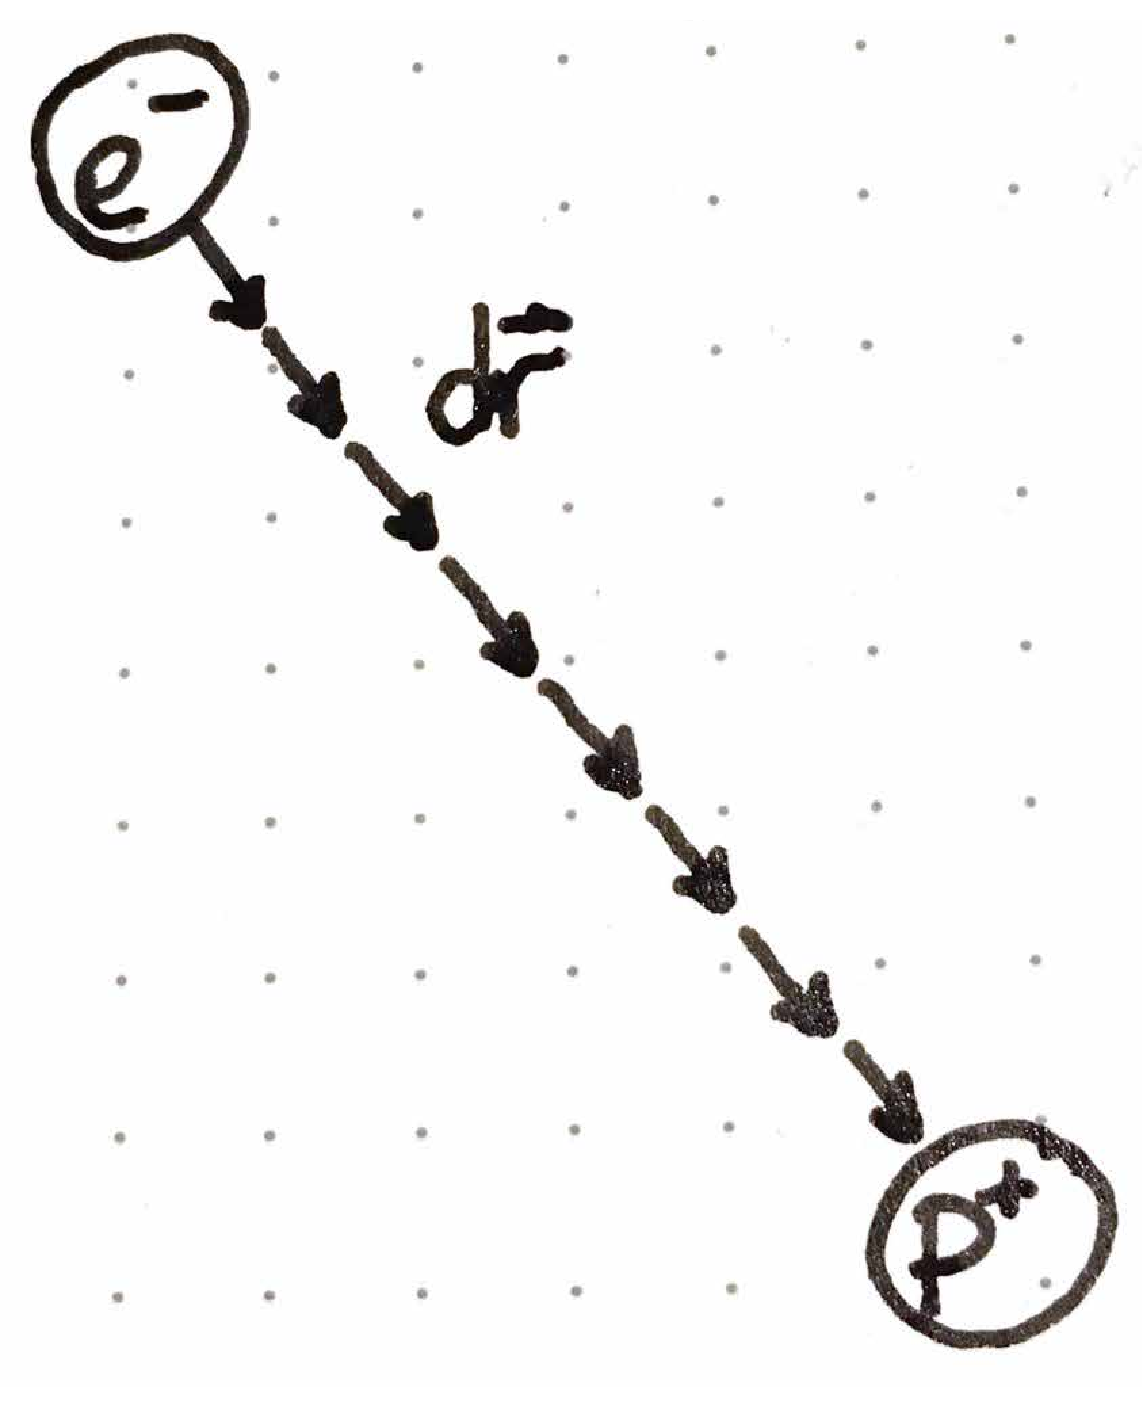
\includegraphics[width=0.6\textwidth]{figures/hydrogen.pdf}
  \end{center}
\end{marginfigure}

On peut calculer le travail effectué par une force en utilisant la relation
\[W = \vF \cdot \Delta\vec{r}\]
seulement lorsque la trajectoire est rectiligne et que la force est constante.
Nous approcherons notre électron du proton le long de la droite qui relie les
deux charges de telle sorte que la trajectoire sera rectiligne.
Malheureusement, la force électrique que subit l'électron n'est pas constante.
Plutôt que de traiter du mouvement de l'électron en un bloc, nous pouvons
diviser la trajectoire en plein de petits segments très courts. Si ces segments
sont suffisamment courts, la force ne variera pratiquement par le long d'un tel
segment.

\begin{enumerate}
  \item Considérez un très court segment de longueur $dr$ de la trajectoire de
    l'électron, alors que celui-ci est à une distance $r$ du proton. En
    supposant que la force ne varie pas le long de ce segment, écrivez une
    expression qui donne le
    travail $dW$ effectué par la force électrique lorsque l'électron se déplace
    le long de ce segment.

  \item Le travail total pour emmener l'électron de très loin jusqu'au
    voisinage du proton est simplement la somme des travaux le long de tous les
    petits segments de trajectoire. Écrivez l'intégrale correspondante et
    résolvez-la.
    \marginnote{Rappel: $\int du/u^2 = -1/u + \text{constante}$.}
\end{enumerate}

\end{document}
